\documentclass[a4paper, 11pt]{article}
\usepackage{graphicx}
\graphicspath{ {./} }
\usepackage{amsmath, nccmath}

\title{Relazione Progetto Programmazione Avanzata}
\author{Kevin Bernardi Matr. n.1058019}
\date{}
\begin{document}
\maketitle
\section{Progetto C++}
\subsection{Introduzione}
Il progetto sulla parte di C++ consiste in una piccola applicazione per tenere traccia di squadre, giocatori, allenatori e delle loro statistiche per il popolare videogioco online competitivo \textit{"Counter Strike: Global Offensive"}, noto anche con l'abbreviazione \textit{"CS:GO"} o \textit{"CSGO"}.

\subsection{Breve panoramica su CSGO}
CSGO è videogioco competitivo online a squadre di 5 giocatori. Ogni partita si svolge tra due squadre per un massimo di 30 round. 
Ogni partita si divide in 2 tempi da 15 round ciascuno della durata di 1 minuto e 55 secondi.
La squadra che vince un round guadagna 1 punto e la prima che arriva a 16 round vinti si aggiudica la vittoria (alla meglio di 30). Se una squadra vince ogni round del primo tempo (15-0) e il primo round del secondo tempo (16-0) la partita termina. Se entrambe le squadre arrivano a 15 punti (punteggio 15 a 15), si procede ad oltranza con i round supplementari.
All'inizio della partita una squadra ha il ruolo di terrorista (\textbf{T}) mentre l'altra di anti-terrorista (\textbf{CT}). I ruoli assunti dalle squadre rimangono fissi per l'intero tempo. Prima del round 16, prima dell'inizio del secondo tempo, i ruoli vengono invertiti.
Ogni squadra per vincere un round ed aggiudicarsi un punto deve:
\begin{itemize}
\item La squadra T può vincere il round facendo esplodere una bomba che deve essere piazzata o eliminando gli avversari entro lo scadere del tempo. La bomba può essere piazzata una sola volta per round;

\item La squadra CT per vincere deve evitare che esploda la bomba piazzata dall'altra squadra o eliminando tutti gli avversari prima che piazzino la bomba o disinnescando la bomba una volta piazzata.
\end{itemize}



\subsection{Metriche}
Come accennato nell'introduzione, il programma serve a raccogliere le statistiche di giocatori, squadre e allenatori per mostrarne le statistiche ed effettuare dei confronti per determinare ad esempio il miglior giocatore, squadra o allenatore.
I giocatori vengono valutati utilizzando la metrica \textit{\textbf{"Average K/D ratio per match"}} abbreviato come \textit{\textbf{"AvgKD"}} calcolato con la seguente formula:
\begin{displaymath}
AvgKD(p) = \frac{ \sum_{m\in matches} \left(\mfrac{kills(m,p)}{deaths(m,p)}\right)}{\#matches}
\end{displaymath}

dove $matches$ è la lista delle partite giocate, $kills(m,p)$ restituisce il numero di eliminazioni della partita $m$ per il giocatore $p$ e $deaths(m,p)$ analogamente restituisce il numero di morti.
Un valore più elevato di questa metrica corrisponde ad un giocatore migliore.
Per quanto riguarda gli allenatori (coach) viene utilizzata una metrica molto simile chiamata \textit{\textbf{"Coach Rating"}} calcolata con la seguente formula:

\begin{displaymath}
Rating(c) = \frac{ \sum_{m\in matches} \left(\mfrac{\sum_{p\in players(m)} \left(\mfrac{kills(m,p)}{deaths(m,p)}\right)}{\#players}\right)}{\#matches}
\end{displaymath}

dove $players(m)$ è la lista dei giocatori di una partita
che in altri termini è la media sulle partite delle medie dei rapporti uccisioni/morti di ogni giocatore nella partita.

\subsection{Struttura del programma}

Il programma è composto dalle seguenti classi:
\begin{itemize}
\item Organization (rappresenta una squadra)
\item Person (rappresenta una persona)
\item Coach (rappresenta un allenatore)
\item Player (rappresenta un giocatore)
\item Retired (rappresenta una persona che si è ritirata dalle competizioni definitivamente)
\item playerMatch (rappresenta un contenitore con le statistiche di un giocatore in una partita)
\end{itemize}

La relazione tra le classi è rappresentata nel seguente diagramma UML:

\begin{center}
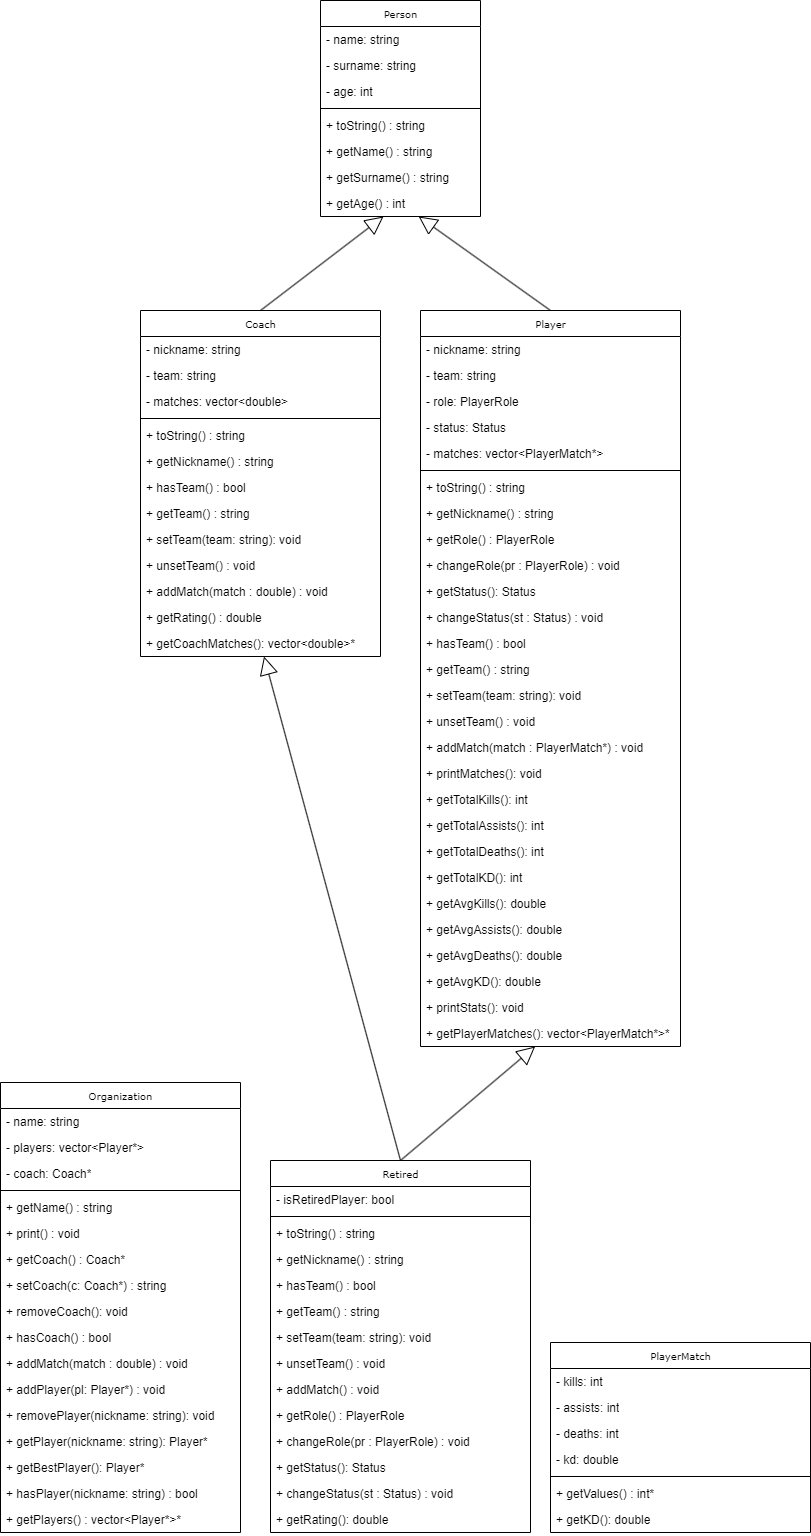
\includegraphics[height=\textheight]{uml}
\end{center}

Il funzionamento dettagliato di ogni classe, funzione, metodo è spiegata all'interno del codice.

\section{Progetto Haskell}
\subsection{Introduzione}
Il progetto in Haskell consiste in un programma che conta le occorrenze delle parole in una pagina web passata come argomento appena dopo aver avviato il programma.
Per realizzare il progetto sono state utilizzate le librerie \textit{"Scalpel"} uno web scraper per estrarre testo dalle pagine web e \textit{"split"} per utilizzare metodi aggiuntivi di manipolazione delle liste come \textit{splitOn()} che consente di dividere una stringa in una lista di sottostringhe per separare le parole contenute nelle frasi.



\end{document}

